\documentclass{article}

% Paquetes plantilla
\usepackage[square, numbers, sort]{natbib}
% \usepackage{cite}
\usepackage{graphicx}
\usepackage[utf8]{inputenc}
\usepackage{amsmath,amssymb,amsfonts}
\usepackage{algorithmic}
\usepackage{textcomp}
\usepackage{subfig}
\usepackage{float}
\usepackage{empheq}
\usepackage{mathtools}
\usepackage[spanish]{babel}
\usepackage[paper=a4paper,margin=2.75cm]{geometry}
\usepackage{booktabs} % for tables
\usepackage[colorlinks = true,
            linkcolor = blue,
            urlcolor  = blue,
            citecolor = orange,
            anchorcolor = blue]{hyperref} % for hyperlinks
\usepackage{xcolor} % text colors
% Paquetes extra
\usepackage{subcaption, booktabs, siunitx, tikz}
\usepackage{pgfplots}
\pgfplotsset{compat=1.15}
\usepackage{mathrsfs}
\usetikzlibrary{arrows}
\tikzset{every picture/.style={line width=0.75pt}} %set default line width to 0.75pt 

\sisetup{
    round-mode          = places, % Rounds numbers
    round-precision     = 2, % to 2 places
}

\usepackage{titlesec}

\setcounter{secnumdepth}{4}

\titleformat{\paragraph}
{\normalfont\normalsize\bfseries}{\theparagraph}{1em}{}
\titlespacing*{\paragraph}
{0pt}{3.25ex plus 1ex minus .2ex}{1.5ex plus .2ex}

% Directorio con imagenes
\graphicspath{{./figs/}}

% Cabecera del documento
% ======================================================================

% Titulo
\title{PROYECTO AUTOMATAS}

% Autores
\author{Juan Pablo Sibecas \\ juan.sibecas@gmail.com \\Matias Gaviño\\ matias.linares.g@gmail.com \\ Autómatas y Control Discreto, Facultad de Ingeniería, \\ Universidad Nacional de Cuyo, \\ Mendoza, Argentina}

% Fecha
\date{Junio de 2024}

% Cuerpo del documento
% ======================================================================
\begin{document}

% Comandos definidos por el autor
\renewcommand{\tablename}{Tabla}
% \renewcommand{\color{blue}{#1}}{\azul}

% Crear cabecera
\maketitle

% Resumen
% ======================================================================
\begin{abstract}\label{sec:abstract}

\end{abstract}

\newpage

\section{Introducción} \label{sec:intro}

\section{Desarrollo} \label{sec:desarrollo}
    \subsection{Modelo del Sistema Físico} \label{sec:plantModel}

        \subsubsection{Subsistema de Izaje}
            Segunda ley de Newton del lado tambor:
            \begin{equation} \label{eq:tamborIzaje}
                J_{hd+hEb} \frac{d \omega_{hd}}{dt} = T_{hd}(t) + T_{hEb}(t) - b_{hd} \omega_{hd}(t) - T_{hdl}(t)
            \end{equation}

            Segunda ley de Newton del lado motor:
            \begin{equation} \label{eq:motorIzaje}
                J_{hm+hb} \frac{d \omega_{hm}}{dt} = T_{hm}(t) + T_{hb}(t) - b_{hm} \omega_{hm}(t) - T_{hml}(t)
            \end{equation}

            relacion de transmision
            \begin{equation} \label{eq:transmisionIzaje}
                i_h = \frac{\omega_{hm}(t)}{\omega_{hd}(t)} = \frac{T_{hd}(t)}{T_{hml}(t)}
            \end{equation}

            si reemplazo \ref{eq:transmisionIzaje} en \ref{eq:motorIzaje} y despejo $T_{hd}(t)$

            \begin{equation} \label{eq:Thd}
                T_{hd}(t) = J_{hm+hb} \frac{d \omega_{hd}}{dt} {i_h}^2 - b_{hm} \omega_{hd}(t) {i_h}^2 + i_h (T_{hm}(t) + T_{hb}(t))
            \end{equation}

            reemplazando en \ref{eq:tamborIzaje} y operando se obtiene

            \begin{equation} \label{eq:izajeThdl}
                (J_{hd+hEb} + J_{hm+hb} i_h^2) \frac{d \omega_{hd}}{dt} = - (b_{hd} + b_{hm}i_h^2) \omega_{hd}(t) + i_h (T_{hm}(t) + T_{hb}(t)) + T_{hEb}(t) - T_{hdl}(t)
            \end{equation}

            como $T_{hdl}(t) = F_{hw}(t)*r_{hd}$, $2V_h = r_{hd}*\omega_{hd}(t)$ y $V_h = -\frac{dl_h(t)}{dt}$ y dividiendo por $r_{hd}$:

            \begin{equation} \label{eq:izajeFhw}
                2\frac{(J_{hd+hEb} + J_{hm+hb} i_h^2)}{r_{hd}^2} \frac{d^2 l_h(t)}{dt^2} = - 2\frac{(b_{hd} + b_{hm}i_h^2)}{r_{hd}^2} \frac{d l_h(t)}{dt} - \frac{i_h}{r_{hd}} (T_{hm}(t) + T_{hb}(t)) - \frac{T_{hEb}(t)}{r_{hd}} + F_{hw}(t)
            \end{equation}
            
            Reemplazando por parametros equivalentes:
            
            \begin{equation} \label{eq:izajeEquiv}
                M_{Eh} \ddot{l_h}(t) = - b_{Eh} \dot{l_h}(t) - \frac{i_h}{r_{hd}} (T_{hm}(t) + T_{hb}(t)) - \frac{T_{hEb}(t)}{r_{hd}} + F_{hw}(t)
            \end{equation}

            Donde

            \begin{align} \label{eq:izajeParamsEquiv}
                M_{Eh} = 2\frac{(J_{hd+hEb} + J_{hm+hb} i_h^2)}{r_{hd}^2}\\
                b_{Eh} = 2\frac{(b_{hd} + b_{hm}i_h^2)}{r_{hd}^2}\\
            \end{align}
            

        \subsubsection{Subsistema Carro}
            Segunda ley de Newton del lado tambor:
            \begin{equation} \label{eq:tamborCarro}
                J_{td} \frac{d \omega_{td}(t)}{dt} = T_{td}(t) - b_{td} \omega_{td}(t) - T_{tdl}(t)
            \end{equation}

            Segunda ley de Newton del lado motor:
            \begin{equation} \label{eq:motorCarro}
                J_{tm+tb} \frac{d \omega_{tm}(t)}{dt} = T_{tm}(t) + T_{tb}(t) - b_{tm} \omega_{tm}(t) - T_{tml}(t)
            \end{equation}

            relacion de transmision
            \begin{equation} \label{eq:transmisionCarro}
                i_t = \frac{\omega_{tm}(t)}{\omega_{td}(t)} = \frac{T_{td}(t)}{T_{tml}(t)}
            \end{equation}

            si reemplazo \ref{eq:transmisionCarro} en \ref{eq:motorCarro} y despejo $T_{td}(t)$

            \begin{equation} \label{eq:Ttd}
                T_{td}(t) = J_{tm+tb} \frac{d \omega_{td}(t)}{dt} {i_t}^2 - b_{tm} \omega_{td}(t) {i_t}^2 + i_t (T_{tm}(t) + T_{tb}(t))
            \end{equation}

            Reemplazo \ref{eq:Ttd} en \ref{eq:tamborCarro} y reordeno:

            \begin{equation} \label{eq:carroTtdl}
                (J_{td} + J_{tm+tb}*i_t^2) \frac{d \omega_{td}(t)}{dt} = i_t (T_{tm}(t) + T_{tb}(t)) - (b_{td} + b_{tm}{i_t}^2) \omega_{td}(t) - T_{tdl}(t)
            \end{equation}
        
            Como $\omega_{td}(t) r_{td} = V_{td}(t)$, $F_{tw}(t)r_{td} = T_{tdl}(t)$ y $V_{td}(t) = \frac{d x_{td}}{dt}$ y dividiendo por $r_{td}$:
            
            \begin{equation} \label{eq:carroFtw}
                \frac{(J_{td} + J_{tm+tb}*i_t^2)}{r_{td}^2} \frac{d^2 x_{td}(t)}{dt^2} = - \frac{(b_{td} + b_{tm}{i_t}^2)}{r_{td}^2} \frac{d x_{td}(t)}{dt} + \frac{i_t}{r_{td}} (T_{tm}(t) + T_{tb}(t)) - F_{tw}(t)
            \end{equation}

            Reemplazando por parametros equivalentes se obtiene la ecuacion del tambor del subsistema carro:

            \begin{equation} \label{eq:TamborCarro}
                M_{Etd} \ddot{x_{td}}(t) = - b_{Etd} \dot{x_{td}}(t) + \frac{i_t}{r_{td}} (T_{tm}(t) + T_{tb}(t)) - F_{tw}(t)
            \end{equation}

            La ecuacion de movimiento del carro es:

            \begin{equation} \label{eq:Carro}
                M_t \ddot{x_{t}}(t) = - b_t \dot{x_{t}}(t) + F_{tw}(t) + 2F_{hw}(t)\sin{\theta_l(t)}
            \end{equation}

            Y la fuerza transmitida por el cable del subsistema carro es:

            \begin{equation} \label{eq:fuerzaCableCarro}
                F_{tw}(t) = K_{tw}(x_{td}(t) - x_t(t)) + b_{tw}(\dot{x_{td}}(t) - \dot{x_t}(t))
            \end{equation}

            seria un sistema acoplado? preguntar si se resuelve asi

                
        \subsection{Diseño del controlador}

            \begin{equation}\label{eq:PID}
                T_m'(t) = b_ae_\omega(t) + K_{sa} e_\theta(t) + K_{sia}\int e_\theta(t) dt
            \end{equation}
            Por lo tanto, por Laplace:
            \begin{equation}\label{eq:PID_Laplace}
                T_m(s) = G(s)[b_aE_\omega(s) + K_{sa} \frac{1}{s} + K_{sia} \frac{1}{s^2}]E_\theta(s)
            \end{equation}

            Donde \(G_T(s)\) es la función de transferencia del modulador de torque que, como se supone ideal, es igual a 1.


            Para obtener la expresión que nos permita obtener las constante que definen al controlador se remplaza la ecuacion \ref{eq:PID} en la ecuacion de movimiento del izaje y del carro, se obtiene:
            Para el izaje, reemplazando \ref{eq:PID} en \ref{eq:izajeEquiv} y transformandola con Laplace, se obtiene:
            \begin{equation}\label{eq:izajeControl}
                M_{Eh} \ddot{L_h}(s) = - b_{Eh} sL_h(s) - \frac{i_h}{r_{hd}} [G(s)[b_aE_\omega(s) + K_{sa} \frac{1}{s} + K_{sia} \frac{1}{s^2}]E_\theta(s)] + F_{hw}(s)
            \end{equation}
            despejando 


            \subsubsection{Control de balanceo}
                Se deducen las ecuaciones de movimiento del sistema carro-péndulo, se obtiene:

                Planteando el equilibrio dinámico de los torques en el anclaje del péndulo:
                \begin{equation}
                    \sum \tau = I \ddot{\theta}
                \end{equation}
                \begin{equation}
                    m l^2 \ddot{\theta} = - m g \sin{\theta} + m \cos{\theta} \ddot{x}_t
                \end{equation}
                despejando \(\ddot{\theta}\):
                \begin{equation}
                    \ddot{\theta} = \frac{\cos{\theta} \ddot{x}_t}{l} - \frac{g \sin{\theta}}{l}
                \end{equation}

                También:
                \begin{equation}
                    x_l = \sin(\theta) l + x_t
                \end{equation}
                \begin{equation}
                    \dot{x}_l = \cos(\theta) \dot{\theta} l + \dot{x}_t
                \end{equation}

                Se definen el vector de estado como:
                \begin{equation}
                    x = \begin{bmatrix}
                        \theta \\
                        \dot{\theta}
                    \end{bmatrix}
                \end{equation}
                \begin{equation}
                    u = \ddot{x}_t
                \end{equation}
                \begin{equation}
                    y = \dot{x}_l
                \end{equation}

                Por lo tanto se expresa el modelo del sistema en el espacio de estados no lineal:
                \begin{equation}
                    \begin{cases}
                        \dot{x} = f(x,u,t) ; x(0) = x_0 \\
                        y = h(x,u,t)
                    \end{cases}
                \end{equation}
                Donde:
                \begin{equation}
                    f(x,u,t) = \begin{bmatrix}
                        \dot{\theta} \\
                        \frac{\cos{\theta} u}{l} - \frac{g \sin{\theta}}{l}
                    \end{bmatrix}
                \end{equation}
                \begin{equation}
                    h(x,u,t) = \cos{\theta} \dot{\theta} l
                \end{equation}
                Se ignora \(\dot{x}_t\) dado que buscaremos el incremendo de velocidad que debemos aplicar al carro para que el péndulo se mantenga en equilibrio.

                Se linealiza el sistema en torno a un punto de trabajo \(x(t), u(t)\) y se obtiene:
                \begin{equation}
                    \begin{cases}
                        \dot{x} = A x + B u \\
                        y = C x + D u
                    \end{cases}
                \end{equation}
                Donde:
                \begin{equation}
                    A_{ij}= \frac{\partial f_i}{\partial x_j} \Bigg|_{x(t), u(t)}
                \end{equation}
                \begin{equation}
                    B_{ij}= \frac{\partial f_i}{\partial u_j} \Bigg|_{x(t), u(t)}
                \end{equation}
                \begin{equation}
                    C_{ij}= \frac{\partial h_i}{\partial x_j} \Bigg|_{x(t), u(t)}
                \end{equation}
                \begin{equation}
                    D_{ij}= \frac{\partial h_i}{\partial u_j} \Bigg|_{x(t), u(t)}
                \end{equation}

                Se obtiene:
                \begin{equation}
                    A = \begin{bmatrix}
                        0 & 1 \\
                        -\cos{\theta}\frac{g}{l^2}-\sin{\theta}\frac{\ddot{x}_t}{l^2} & 0
                    \end{bmatrix}
                \end{equation}
                \begin{equation}
                    B = \begin{bmatrix}
                        0 \\
                        \frac{\cos{\theta}}{l^2}
                    \end{bmatrix}
                \end{equation}
                \begin{equation}
                    C = \begin{bmatrix}
                        -\sin{\theta}\dot{\theta}l & \cos{\theta}l
                    \end{bmatrix}
                \end{equation}
                \begin{equation}
                    D = 0
                \end{equation}

                Se propone un controlador PD para el sistema:
                \begin{equation}
                    u =  K_p (y^*-y) + K_d \frac{d}{dt}(y^*-y)
                \end{equation}

                \begin{equation}
                    \dot{x} = A x + B ( K_p (y^*-y) + K_d \frac{d}{dt}(y^*-y))
                \end{equation}
                \begin{equation}
                    \dot{x} = A x + B ( K_p (y^*-C x) + K_d \frac{d}{dt}(y^*-C x))
                \end{equation}

                \begin{equation}
                    \ddot{\theta} = A_{21} \dot{\theta} + B_{2} ( K_p (\dot{x}_l^*-C_1\theta-C_2\dot{\theta}) + K_d \frac{d}{dt}(\dot{x}_l^*-C_1\theta-C_2\dot{\theta}))
                \end{equation}
                \begin{equation}
                    \ddot{\theta} = A_{21} \theta + B_{2} K_p \dot{x}_l^* - B_{2} K_p C_1 \theta - B_{2} K_p C_2 \dot{\theta} + \frac{d}{dt} \left( B_{2} K_d \dot{x}_l^* - B_{2} K_d C_1 \theta - B_{2} K_d C_2 \dot{\theta} \right)
                \end{equation}
                Utilizando la transformada de Laplace:
                \begin{equation}
                    s^2 \Theta = A_{21} \Theta + B_{2} K_p \dot{X}_l^* - B_{2} K_p C_1 \Theta - B_{2} K_p C_2 s \Theta + B_{2} K_d \dot{X}_l^*s - B_{2} K_d C_1 \Theta s - B_{2} K_d C_2 \Theta s^2
                \end{equation}
                Despejando \(\theta/\dot{X}_l^*\):
                \begin{equation}
                    \Theta( s^2(B_{2} K_d C_2) + s (B_{2} K_p C_2 - B_{2} K_d C_1) - A_{21} + B_{2} K_p C_1) = \dot{X}_l^* (B_{2} K_p + B_{2} K_d s)
                \end{equation}

                \begin{equation} \label{eq:thetaXl}
                    \frac{\theta}{\dot{X}_l^*}= \frac{B_{2} K_p + B_{2} K_d s}{s^2(B_{2} K_d C_2) + s (B_{2} K_p C_2 - B_{2} K_d C_1) - A_{21} + B_{2} K_p C_1}
                \end{equation}

                Se obtinen las constantes \(K_p\) y \(K_d\) de forma que el denominado de \ref{eq:thetaXl} cumpla \(s^2 + s 2 \eta \omega + \omega^2 = 0\)

                \begin{equation}
                    \begin{cases}
                        2 \eta \omega = \frac{B_{2} K_p C_2 - B_{2} K_d C_1 }{B_{2} K_d C_2} \\
                        \omega^2 = \frac{A_{21} - B_{2} K_p C_1}{B_{2} K_d C_2}
                    \end{cases}
                \end{equation}
                \begin{equation}
                    \begin{cases}
                        2 \eta \omega = \frac{K_p}{K_d}-\frac{C_1 }{C_2} \\
                        \omega^2 = \frac{A_{21}}{B_{2} K_d C_2} - \frac{K_p C_1}{K_d C_2}
                    \end{cases}
                \end{equation}

                \begin{equation}
                    \begin{cases}
                        2 \eta \omega K_d=  K_p - K_d \frac{C_1 }{C_2} \\
                        \omega^2 K_d = \frac{A_{21}}{B_{2} C_2} - K_p \frac{C_1}{C_2}
                    \end{cases}
                \end{equation}

                \begin{equation}
                    \begin{cases}
                        K_p + K_d (-\frac{C_1}{C_2} - 2 \eta \omega) = 0 \\
                        K_p \frac{C_1}{C_2} + K_d \omega^2 = \frac{A_{21}}{B_{2} C_2} 
                    \end{cases}
                \end{equation}

                \begin{equation}
                    \begin{cases}
                        K_p = \frac{\frac{A_{21}}{B_{2} C_2}}{\omega^2-(-\frac{C_1}{C_2} - 2 \eta \omega)\frac{C_1}{C_2}} \\
                        K_d = \frac{-\frac{A_{21}}{B_{2} C_2} (-\frac{C_1}{C_2} - 2 \eta \omega)}{\omega^2-(-\frac{C_1}{C_2} - 2 \eta \omega)\frac{C_1}{C_2}}
                    \end{cases}
                \end{equation}

                \begin{equation}
                    \begin{cases}
                        K_p = \frac{\frac{A_{21}}{B_{2} C_2}}{\omega^2+(\frac{C_1}{C_2} + 2 \eta \omega)\frac{C_1}{C_2}} \\
                        K_d = \frac{\frac{A_{21}}{B_{2} C_2} (\frac{C_1}{C_2} + 2 \eta \omega)}{\omega^2+(\frac{C_1}{C_2} + 2 \eta \omega)\frac{C_1}{C_2}}
                    \end{cases}
                \end{equation}





\subsubsection{Control de balanceo}

            A continuación se derivan las ecuaciones que modelan el sistema carro-pendulo. Se utilizará el metodo de Lagrange definiendo las cordenadas generalizadas 
            \(x_t\) y \(\theta\) . Donde \(x_t\) es la posición del carro y \(\theta\) es el angulo del pendulo respecto a la vertical. 
            A modo de simplificaion se toma \(l\) como un parametro y no como una funcion del tiempo.
            El sistema se modela siguiento el modelo físico de la figura 3 del enunciado.
            \begin{figure}[H]
                \centering
                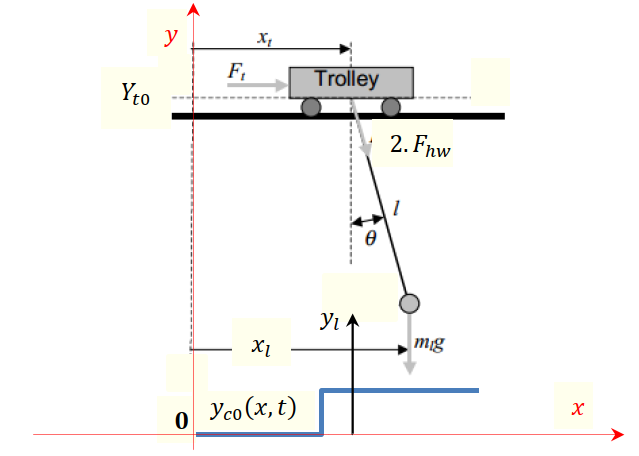
\includegraphics[width=0.5\textwidth]{figs/figure3_enunciado.png}
                \caption{Modelo físico simplificado del subsistema Carro – Cable – Carga y Perfil de Obstáculos}
                \label{fig:pendulo}
            \end{figure}
            
            \begin{equation}\label{eq:kinetic1}
                K = K_t + K_{lx} + K_{ly}
            \end{equation}
            \begin{equation}\label{eq:xl}
                x_l=x_t+l\sin{\theta}
            \end{equation}
            \begin{equation}\label{eq:dxl}
                \dot{x_l}=\dot{x_t}+l\cos{\theta}\dot{\theta}
            \end{equation}
            \begin{equation}\label{eq:y}
                y_l=Y_{t0}-l\cos{\theta}
            \end{equation}
            \begin{equation}\label{eq:dy}
                \dot{y_l}=-l\sin{\theta}\dot{\theta}
            \end{equation}

            \begin{equation}\label{eq:kinetic2}
                K = \frac{1}{2}m_t\dot{x_t}^2   +\frac{1}{2}m_l\dot{x_l}^2  +\frac{1}{2}m_l\dot{y_l}^2
            \end{equation}

            \begin{equation}\label{eq:kinetic3}
                K = \frac{1}{2}m_t\dot{x_t}^2   +\frac{1}{2}m_l(\dot{x_t}+l\cos{\theta}\dot{\theta})^2  +\frac{1}{2}m_l(-l\sin{\theta}\dot{\theta})^2
            \end{equation}

            \begin{equation}\label{eq:kinetic4}
                    K = \frac{1}{2}m_t\dot{x_t}^2 +\frac{1}{2}m_l(\dot{x_t}^2+l^2\cos^2{\theta}\dot{\theta}^2
                    +2l\dot{x_t}\cos{\theta}\dot{\theta})+\frac{1}{2}m_ll^2\sin^2{\theta}\dot{\theta}^2
            \end{equation}

            \begin{equation}\label{eq:potential}
                U = -m_lgl\cos{\theta}
            \end{equation}
            \begin{equation}\label{eq:lagrange}
                L = K - U
            \end{equation}

            \begin{equation}\label{eq:lagrange2}
                    L = \frac{1}{2}m_t\dot{x_t}^2
                    +\frac{1}{2}m_l(\dot{x_t}^2
                +l^2\cos^2{\theta}\dot{\theta}^2
                +2l\dot{x_t}\cos{\theta}\dot{\theta})
                +\frac{1}{2}m_ll^2\sin^2{\theta}\dot{\theta}^2
                +m_lgl\cos{\theta}
            \end{equation}

            \begin{equation}\label{eq:lagrange3}
                L = \frac{1}{2}m_t\dot{x_t}^2+\frac{1}{2}m_l\dot{x_t}^2
                +\frac{1}{2}m_ll^2\dot{\theta}^2
                +m_l\dot{x_t}l\cos{\theta}\dot{\theta}
                +m_lgl\cos{\theta}
            \end{equation}

            Se define el sistema de ecuaciones de Euler-Lagrange:
            \begin{equation}\label{eq:euler1}
                \frac{d}{dt}\left(\frac{\partial L}{\partial \dot{q}_i}\right)-\frac{\partial L}{\partial q_i}=Q_i
            \end{equation}

            Para \(q_i = x_t\):
            \begin{equation}\label{eq:euler2}
                \frac{d}{dt}\left(\frac{\partial L}{\partial \dot{x}_t}\right)-\frac{\partial L}{\partial x_t}=Q_t
            \end{equation}
            \begin{equation}
                \frac{\partial L}{\partial \dot{x}_t}= (m_t+m_l)\dot{x}_t+m_ll\cos{\theta}\dot{\theta}
            \end{equation}
            \begin{equation}            
                    \frac{d}{dt}\left(\frac{\partial L}{\partial \dot{x}_t}\right)= 
                    (m_t+m_l)\ddot{x}_t+m_l l\cos{\theta}\ddot{\theta}-m_ll\sin{\theta}\dot{\theta}^2
            \end{equation}
            \begin{equation}
                \frac{\partial L}{\partial x_t}=0
            \end{equation}
            Entonces:
            \begin{equation}
                (m_t+m_l)\ddot{x}_t+m_l l\cos{\theta}\ddot{\theta}-m_l l\sin{\theta}\dot{\theta}^2=F_t(t)-b_{eqt} \dot{x}_t
            \end{equation}

            Para \(q_i = \theta\):

            \begin{equation}\label{eq:euler3}
                \frac{d}{dt}\left(\frac{\partial L}{\partial \dot{\theta}}\right)-\frac{\partial L}{\partial \theta}=Q_{\theta}
            \end{equation}

            \begin{equation}
                \frac{\partial L}{\partial \dot{\theta}}=m_l\dot{x_t}l\cos{\theta}+m_ll^2\dot{\theta}
            \end{equation}

            \begin{equation}
                    \frac{d}{dt}\left(\frac{\partial L}{\partial \dot{\theta}}\right)= m_l\ddot{x_t}l\cos{\theta} -m_l\dot{x_t}l\sin{\theta}\dot{\theta}+m_ll^2\ddot{\theta}
            \end{equation}

            \begin{equation}
                \frac{\partial L}{\partial \theta}=-m_l\dot{x_t}l\sin{\theta}\dot{\theta}-m_lgl\sin{\theta}
            \end{equation}

            Entonces:
            \begin{equation}
                m_l\ddot{x_t}l\cos{\theta} -m_l\dot{x_t}l\sin{\theta}\dot{\theta}+m_ll^2\ddot{\theta}+m_l\dot{x_t}l\sin{\theta}\dot{\theta}+m_lgl\sin{\theta}=0
            \end{equation}

            Finalmente, el sistema de ecuaciones que define el modelo del sistema carro-pendulo es:
            \begin{equation}
                \begin{cases}
                    (m_t+m_l)\ddot{x}_t+m_ll\cos{\theta}\ddot{\theta}-m_ll\sin{\theta}\dot{\theta}^2=F_t(t)-b_{eqt} \dot{x}_t\\
                    m_l\ddot{x_t}l\cos{\theta} -m_l\dot{x_t}l\sin{\theta}\dot{\theta}+m_ll^2\ddot{\theta}+m_l\dot{x_t}l\sin{\theta}\dot{\theta}+m_lgl\sin{\theta}=0
                \end{cases}
            \end{equation}

            \begin{empheq}[box=\fbox]{equation}
                \begin{cases}
                    (m_t+m_l)\ddot{x}_t + m_l l \cos{\theta} \ddot{\theta} - m_l l \sin{\theta} \dot{\theta}^2 = 0 \\
                    \ddot{x}_t \cos{\theta} + l \ddot{\theta} + g \sin{\theta} = 0
                \end{cases}
            \end{empheq}


            Para representar lo en el espacio de estados se definen las siguientes variables de estado \(x\) y entradas \(u\):
            \begin{equation}
                x = \begin{bmatrix}
                    \theta \\
                    \dot{\theta}
                \end{bmatrix}
            \end{equation}
            \begin{equation}
                u = \ddot{x_l}
            \end{equation}

            Entonces, se obtiene el siguiente modelo en el espacio de estados no lineal:

            \begin{equation}
                \begin{cases}
                    \dot{x} = f(x,u,t) ; x(0) = x_0 \\
                    y = h(x,u,t)
                \end{cases}
            \end{equation}



        \subsubsection{Control de balanceo}
            \begin{equation}
                U=\ddot{X}_t= \left(b_a s+k_{sa}\right) \left(X_l^*- X_l\right)
            \end{equation}
            \begin{equation}
                \left(X_l^*- X_l\right)= \frac{1}{s}\left(\dot{X}_l^*- \dot{X}_l\right)
            \end{equation}

            \begin{equation}
                U=\ddot{X}_t= \left(b_a+k_{sa}\frac{1}{s}\right) \left(\dot{X}_l^*- \dot{X}_l\right)
            \end{equation}

            \begin{equation}
                s^2 \Theta = A_{21} \Theta + B_{2} \left( \left(b_a+k_{sa}\frac{1}{s}\right) \left(\dot{X}_l^*- C_1 \Theta-C_2 \Theta s - \dot{X}_t\right) \right)
            \end{equation}

            \begin{equation}
                \begin{split}
                s^2 \Theta = A_{21} \Theta + B_{2} \biggl(  b_a\left(\dot{X}_l^*- C_1 \Theta -C_2 \Theta s + \dot{X}_t\right) + k_{sa}\frac{1}{s}\left(\dot{X}_l^* -C_1 \Theta -C_2 \Theta s - \dot{X}_t\right)\biggr)
                \end{split}
            \end{equation}

            \begin{equation}
                \begin{split}
                s^2 \Theta = A_{21} \Theta + B_{2}\biggl(  b_a\dot{X}_l^*- b_a C_1 \Theta -b_a C_2 \Theta s + k_{sa}\dot{X}_l^*\frac{1}{s} - k_{sa} C_1 \Theta \frac{1}{s} - k_{sa} C_2 \Theta \\
                - \dot{X}_t\left(b_a+k_{sa}\frac{1}{s}\right)\biggr)
                \end{split}
            \end{equation}

            \begin{equation}
                \begin{split}
                s^2 \Theta = A_{21} \Theta + B_{2}b_a\dot{X}_l^*- B_{2}b_a C_1 \Theta -B_{2}b_a C_2 \Theta s + B_{2}k_{sa}\dot{X}_l^*\frac{1}{s} - B_{2}k_{sa} C_1 \Theta \frac{1}{s} - B_{2}k_{sa} C_2 \Theta \\
                - B_{2}\dot{X}_t\left(b_a+k_{sa}\frac{1}{s}\right)
                \end{split}
            \end{equation}

            \begin{equation}
                \begin{split}
                \Theta s^3 =  A_{21} \Theta s + B_{2}b_a \dot{X}_l^* s- B_{2}b_a C_1 \Theta s -B_{2}b_a C_2 \Theta s^2 + B_{2}k_{sa} \dot{X}_l^* - B_{2}k_{sa} C_1 \Theta - B_{2}k_{sa} C_2 \Theta s \\
                - B_{2}\dot{X}_t\left(b_a s+k_{sa}\right)
                \end{split}
            \end{equation}

            \begin{equation}
                \begin{split}
                0= \Theta \left( s^3 + s^2 \left(B_{2}b_a C_2\right) + s \left(-A_{21} +B_{2}b_a C_1 +B_{2}k_{sa} C_2 \right) + \left( B_{2}k_{sa} C_1 \right) \right)\\
                - \dot{X}_l^*\left(B_{2}b_a s + B_{2}k_{sa}\right) +\dot{X}_t\left(B_{2}b_a s+B_{2}k_{sa}\right)   
                \end{split}
            \end{equation}


            \begin{equation}
                \begin{split}
                    \Theta= \frac{B_{2}b_a s + B_{2}k_{sa}}{s^3 + s^2 \left(B_{2}b_a C_2\right) + s \left(-A_{21} +B_{2}b_a C_1 +B_{2}k_{sa} C_2 \right) + \left( B_{2}k_{sa} C_1 \right)} \dot{X}_l^*\\
                    - \frac{B_{2}b_a s+B_{2}k_{sa}}{s^3 + s^2 \left(B_{2}b_a C_2\right) + s \left(-A_{21} +B_{2}b_a C_1 +B_{2}k_{sa} C_2 \right) + \left( B_{2}k_{sa} C_1 \right)} \dot{X}_t
                \end{split}
            \end{equation}

            \begin{equation}
                p_r(s)=(s+\omega_n)(s^2+2\zeta\omega_n s+\omega_n^2)
            \end{equation}
            \begin{equation}
                p_r(s)=s^3+\omega_n(2\zeta+1)s^2+\omega_n^2(2\zeta+1)s +\omega_n^3
            \end{equation}
            \begin{equation}
                p_r(s)=s^3+\omega_n \eta s^2+\omega_n^2 \eta s +\omega_n^3
            \end{equation}

            \begin{equation}
                \begin{cases}
                    \omega_n^3 = B_{2}k_{sa} C_1 \\
                    \omega_n^2 \eta = -A_{21} +B_{2}b_a C_1 +B_{2}k_{sa} C_2 \\
                    \omega_n \eta  = B_{2}b_a C_2 
                \end{cases}
            \end{equation}

            SI \(C_1=0\).

            \begin{equation}
                \begin{split}
                    \Theta= \frac{B_{2}b_a s + B_{2}k_{sa}}{s\left(s^2 + s \left(B_{2}b_a C_2\right) + \left(-A_{21} +B_{2}k_{sa} C_2 \right)\right)} \dot{X}_l^*\\
                    - \frac{B_{2}b_a s+B_{2}k_{sa}}{s\left(s^2 + s \left(B_{2}b_a C_2\right) + \left(-A_{21} +B_{2}k_{sa} C_2 \right)\right)} \dot{X}_t
                \end{split}
            \end{equation}

        \subsubsection{Control de balanceo}
            \begin{equation}
                U=\ddot{X}_t= \left(b_a s+k_{sa}\right) \left(\dot{X}_l^*- \dot{X}_l\right)
            \end{equation}
            
            \begin{equation}
                s^2 \Theta = A_{21} \Theta + B_{2} \left( \left(b_a s+k_{sa}\right) \left(\dot{X}_l^*- C_1 \Theta-C_2 \Theta s - \dot{X}_t\right) \right)
            \end{equation}

            \begin{equation}
                \begin{split}
                s^2 \Theta = A_{21} \Theta + B_{2} \biggl(  b_a s\left(\dot{X}_l^*- C_1 \Theta -C_2 \Theta s + \dot{X}_t\right) + k_{sa}\left(\dot{X}_l^* -C_1 \Theta -C_2 \Theta s - \dot{X}_t\right)\biggr)
                \end{split}
            \end{equation}

            \begin{equation}
                \begin{split}
                s^2 \Theta = A_{21} \Theta + B_{2}\biggl(  b_a \dot{X}_l^* s- b_a C_1 \Theta s-b_a  C_2 \Theta s^2 + k_{sa}\dot{X}_l^* - k_{sa} C_1 \Theta - k_{sa} C_2 \Theta s\\
                - \dot{X}_t\left(b_a s+k_{sa}\right)\biggr)
                \end{split}
            \end{equation}

            \begin{equation}
                \begin{split}
                s^2 \Theta = A_{21} \Theta + B_{2}b_a\dot{X}_l^* s - B_{2}b_a C_1 \Theta s-B_{2}b_a C_2 \Theta s^2 + B_{2}k_{sa}\dot{X}_l^* - B_{2}k_{sa} C_1 \Theta  - B_{2}k_{sa} C_2 \Theta s\\
                - B_{2}\dot{X}_t\left(b_a+k_{sa}\frac{1}{s}\right)
                \end{split}
            \end{equation}

            \begin{equation}
                \begin{split}
                0= \Theta \left( s^2 \left(1+B_{2}b_a C_2\right) + s \left( B_{2}b_a C_1 +B_{2}k_{sa} C_2 \right) + \left( B_{2}k_{sa} C_1 \right) \right)\\
                - \dot{X}_l^*\left(B_{2}b_a s + B_{2}k_{sa}\right) +\dot{X}_t\left(B_{2}b_a s+B_{2}k_{sa}\right)
                \end{split}
            \end{equation}


            \begin{equation}
                \begin{split}
                    \Theta= \frac{B_{2}b_a s + B_{2}k_{sa}}{ s^2 \left(1+B_{2}b_a C_2\right) + s \left( B_{2}b_a C_1 +B_{2}k_{sa} C_2 \right) + \left( B_{2}k_{sa} C_1 \right)} \dot{X}_l^*\\
                    - \frac{B_{2}b_a s+B_{2}k_{sa}}{ s^2 \left(1+B_{2}b_a C_2\right) + s \left( B_{2}b_a C_1 +B_{2}k_{sa} C_2 \Theta \right) + \left( B_{2}k_{sa} C_1 \right)} \dot{X}_t
                \end{split}
            \end{equation}

            \begin{equation}
                p_r(s)=s^2 + s \frac{B_{2}b_a C_1 +B_{2}k_{sa} C_2 }{1+B_{2}b_a C_2} + \frac{B_{2}k_{sa} C_1}{1+B_{2}b_a C_2}
            \end{equation}
            \begin{equation}
                p_r(s)=(s^2+2\zeta\omega_n s+\omega_n^2)
            \end{equation}

            \begin{equation}
                \begin{cases}
                    2\zeta\omega_n = \frac{B_{2}b_a C_1 +B_{2}k_{sa} C_2 }{1+B_{2}b_a C_2} \\
                    \omega_n^2 = \frac{B_{2}k_{sa} C_1}{1+B_{2}b_a C_2}
                \end{cases}
            \end{equation}

            \begin{equation}
                \begin{cases}
                    (1+B_{2}b_a C_2)2\zeta\omega_n = B_{2}b_a C_1 +B_{2}k_{sa} C_2\\
                    (1+B_{2}b_a C_2)\omega_n^2 = B_{2}k_{sa} C_1
                \end{cases}
            \end{equation}

            \begin{equation}
                \begin{cases}
                    2\zeta\omega_n+ 2\zeta\omega_n B_{2}b_a C_2 = B_{2}b_a C_1 +B_{2}k_{sa} C_2\\
                    \omega_n^2+B_{2}b_a C_2\omega_n^2= B_{2}k_{sa} C_1
                \end{cases}
            \end{equation}

            \begin{equation}
                \begin{cases}
                    b_a(2\zeta\omega_n B_{2}C_2-B_{2}C_1) &+ k_{sa}(-B_{2}C_2) = -2\zeta\omega_n \\
                    b_a(\omega_n^2B_{2}C_2) &+ k_{sa}(-B_{2}C_1) = -\omega_n^2
                \end{cases}
            \end{equation}

            




                    

                




\section{Resultados}\label{sec:results}

\section{Conclusión}\label{sec:conclusion}


% Estilo de citas
%\bibliographystyle{unsrt}

% Nombre del archivo .bib
%\bibliography{references}

\end{document}